\documentclass{sigchi}

% Use this command to override the default ACM copyright statement
% (e.g. for preprints).  Consult the conference website for the
% camera-ready copyright statement.

%% EXAMPLE BEGIN -- HOW TO OVERRIDE THE DEFAULT COPYRIGHT STRIP -- (July 22, 2013 - Paul Baumann)
% \toappear{Permission to make digital or hard copies of all or part of this work for personal or classroom use is      granted without fee provided that copies are not made or distributed for profit or commercial advantage and that copies bear this notice and the full citation on the first page. Copyrights for components of this work owned by others than ACM must be honored. Abstracting with credit is permitted. To copy otherwise, or republish, to post on servers or to redistribute to lists, requires prior specific permission and/or a fee. Request permissions from permissions@acm.org. \\
% {\emph{CHI'14}}, April 26--May 1, 2014, Toronto, Canada. \\
% Copyright \copyright~2014 ACM ISBN/14/04...\$15.00. \\
% DOI string from ACM form confirmation}
%% EXAMPLE END -- HOW TO OVERRIDE THE DEFAULT COPYRIGHT STRIP -- (July 22, 2013 - Paul Baumann)

% Arabic page numbers for submission.  Remove this line to eliminate
% page numbers for the camera ready copy 
% \pagenumbering{arabic}

% Load basic packages
\usepackage{balance}  % to better equalize the last page
\usepackage{graphics} % for EPS, load graphicx instead 
%\usepackage[T1]{fontenc}
\usepackage{txfonts}
\usepackage{times}    % comment if you want LaTeX's default font
\usepackage[pdftex]{hyperref}
% \usepackage{url}      % llt: nicely formatted URLs
\usepackage{color}
\usepackage{textcomp}
\usepackage{booktabs}
\usepackage{ccicons}
\usepackage{todonotes}

\usepackage{subcaption}


% llt: Define a global style for URLs, rather that the default one
\makeatletter
\def\url@leostyle{%
  \@ifundefined{selectfont}{\def\UrlFont{\sf}}{\def\UrlFont{\small\bf\ttfamily}}}
\makeatother
\urlstyle{leo}

% To make various LaTeX processors do the right thing with page size.
\def\pprw{8.5in}
\def\pprh{11in}
\special{papersize=\pprw,\pprh}
\setlength{\paperwidth}{\pprw}
\setlength{\paperheight}{\pprh}
\setlength{\pdfpagewidth}{\pprw}
\setlength{\pdfpageheight}{\pprh}

% Make sure hyperref comes last of your loaded packages, to give it a
% fighting chance of not being over-written, since its job is to
% redefine many LaTeX commands.
\definecolor{linkColor}{RGB}{6,125,233}
\hypersetup{%
  pdftitle={SwipeKey: A Swipe-based Keyboard Design For Smartwatches},
  pdfauthor={LaTeX},
  pdfkeywords={SIGCHI, proceedings, archival format},
  bookmarksnumbered,
  pdfstartview={FitH},
  colorlinks,
  citecolor=black,
  filecolor=black,
  linkcolor=black,
  urlcolor=linkColor,
  breaklinks=true,
}

% create a shortcut to typeset table headings
% \newcommand\tabhead[1]{\small\textbf{#1}}

\newcommand{\papertitle}{SwipeKey}

% End of preamble. Here it comes the document.
\begin{document}

\title{SwipeKey: A Swipe-based Keyboard Design For Smartwatches}

\numberofauthors{3}
\author{%
  \alignauthor{1st Author Name\\
    \affaddr{Affiliation}\\
    \affaddr{City, Country}\\
    \email{e-mail address}}\\
  \alignauthor{2nd Author Name\\
    \affaddr{Affiliation}\\
    \affaddr{City, Country}\\
    \email{e-mail address}}\\
  \alignauthor{3rd Author Name\\
    \affaddr{Affiliation}\\
    \affaddr{City, Country}\\
    \email{e-mail address}}\\
}

\maketitle

\begin{abstract}

The rise of smartwatches calls for efficient, convenient and suitable text input methods for these small computers. The minuscule size of these screen brings many challenges in how users interact with these devices. Although tech savvy and casual users alike are all familiar with the ubiquitous QWERTY keyboard layout found on most computer keyboards, smartphones, and tablets, this layout cannot fit on small, wearable devices. We introduce \papertitle\, a text input method that uses swipe directions to allow multiple inputs per button and thus allow for an increase in the effective size of input buttons. We have conducted thorough experiments to optimize \papertitle\ to enable a fast, low-error, and easy to learn keyboard for smartwatches. These benefits result from having a keyboard that emphasizes the use of swipe motions. Our user study results show that with a specific combination of swipe direction identification (such as up, down, left, right, and diagonal swipe directions) and its corresponding button size (big, medium, and small button sizes), \papertitle\ users achieved an 55\% improvement in words per minute (WPM) and dramatically decreased error rate by 44\% compared to other text input methods designed for small screens.

\end{abstract}

\category{H.5.2}{Information interfaces and presentation:}{User Interfaces - Graphical user interfaces; Input devices and strategies.} \category{}{}{}

\keywords{Text entry, input, smartwatch, \papertitle, keyboard design}

\section{Introduction}
Smartwatches have become more and more popular in the consumer market. There are many recently released products such as the Apple Watch \cite{apple-watch}, LG Watch Urbane \cite{lg-urban}, Samsung Gear S \cite{samsung-gear-s}, Sony SmartWatch 3 \cite{sony-sw3}, Pebble Time \cite{pebble-time}, and Moto360 \cite{moto360} that are more powerful and power efficient than ever before and make smartwatches much more capable and practical than prior models. 
Smartwatches rely on small touchscreens and voice recognition for input. Most smartwatches only provide voice input or a selection of predetermined short messages as text entry. Because typing on such a small screen is very difficult with ordinary QWERTY soft-keyboards, a number of solutions to mitigate this problem of text entry on small devices have been proposed. Some of the solution use wristbands, chording, or other sensors  \cite{wristband-text-entry,one-hand-chording,tilt-type,airwriting-on-wearable,mid-air-gesture}, and some work on the design of the keyboard \cite{text-entry-on-small-qwerty,text-entry-for-mobile,zoomboard,1-line-qwerty,splitboard}.

\begin{figure}
  \centering
  \includegraphics[width=1\columnwidth]{figures/F1.jpg}
  \caption{\papertitle\ 4 implemented on Sony SmartWatch 3}
  \label{fig:f1}
\end{figure}

The major issue for smartwatch text entry is the difficulty of using these extremely small screens for touch input. For example: an iPhone 4 has a screen size of 76.65mm x 51.60mm, the Sony SW3 smartwatch has a screen dimension of 28.7mm x 28.7mm. The dimensions of the onscreen keyboard on an iPhone 4 are 51.6mm x 33.5mm, which is still much larger than the entire screen size of the Sony SW3 smartwatch. Furthermore, we cannot reserve the entire screen of the smartwatch to display a software keyboard since it will leave no space to display text as the user is typing. If we fill half of the smartwatche's screen to display an iPhone 4 software keyboard, each of the keyboard buttons would be 4.2 times smaller on the Sony SW3. A tiny keyboard and button size decreases the users input speed and accuracy when the user is typing on a smartwatch keyboard.

When we talk about the “effective” button size, we mean the ease of pressing buttons due to several factors. One factor is size. Obviously, a big button the size of an ordinary computer keyboard is much easier to press than a tiny button that is less than a quarter the size. Buttons that are both small and tightly packed together will also make pressing a specific button difficult. Since smartwatch screens are naturally small, there are few options that would allow for increased button sizes. This is why we need to incorporate other techniques to make the buttons “feel” bigger. Keyboard designers can achieve this by using gestures. Making them “feel” bigger and easier to type makes the “effective” button size bigger without making the buttons physically bigger.

There are a lot of keyboards designated for small screen mobile devices that attempts to increase the effective button size \cite{zoomboard,swipeboard,text-entry-on-small-qwerty}.
They use many different methods to increase the effective size of the keyboard keys.
 However, Luis etal. \cite{text-entry-on-small-qwerty} shows that the proper design for various small-screen mobile can differ for one of them. These works primarily focus on general mobile devices; for smartwatches specifically however, there is still a room to be explored.

In our paper, we focus on designing a keyboard layout that is suitable for most of the commercially available smartwatches. We have designed a keyboard and have optimized and evaluated several parameters crucial for smartwatch keyboard design through our design process and user studies.

Our first contribution is that we implemented \papertitle: a one swipe or tap keyboard for smartwatches. We tried to optimize several crucial parameters and have shown that \papertitle\ can outperform one existing keyboard for small devices in speed, accuracy, learning difficulty, and user preference.

Our second contribution is that we study some of the parameters of keyboard design and touch screen input on smartwatches. We also provide some design principles for keyboards on smartwatches that have proven themselves in our user studies.

\section{Related Work}

\subsection{Voice Input}
Voice input is a popular input method available on most mobile devices. Currently, smartwatches also use voice input. Smartwatches on the market include the Apple Watch, Moto G, Sony SmartWatch 3, Pebble, Samsung Gear S, and Huawei Watch \cite{huawei-watch}. All these smartwatches support voice input for performing a variety of actions. Voice input provides a hand-free and high-speed text entry method to mobile device users \cite{voice-input-mobile,android-speech-recognition}. However, voice input may not be socially acceptable in certain situations. For example, in public spaces, it is not common to see people using their device with voice control. Furthermore, users may find voice input unreliable in regards to speech recognition accuracy. Voice recognition is not perfect, especially when the quality of the users’ voice or accent and ambient sounds in the environment negatively affect the output. Therefore, to make text entry reliable across different scenarios, an alternative text input method is necessary for smartwatches.

\subsection{Software Keyboard}
Since smartphone users are accustomed to using touchscreen keyboards, software keyboard designers naturally want to find ways of fitting keyboards onto smartwatches.

\subsubsection{ZoomBoard}
ZoomBoard \cite{zoomboard}, designed by Carnegie Mellon University \& Friendship House, is designed for small mobile devices. ZoomBoard maps QWERTY soft-keyboard onto the display. ZoomBoard zooms in on the keyboard area that the user tapped on. On this now enlarged section of the keyboard, the user can tap on a specific button to type the selected character. The keyboard will then zoom out to its original size. Since zoom navigation is common on smartphones, users will find ZoomBoard easy to learn as it does not require users to memorize any kind of special input techniques. This text entry method is designed for small screen devices and it is shown to be more suitable for small screens instead of medium or large screen sizes.\cite{text-entry-on-small-qwerty}

\subsubsection{Swipeboard}
Swipeboard \cite{swipeboard}, by Autodesk Research, is another software keyboard made for small devices. The 2 swipe or tap text input method is shown to outperform ZoomBoard after less than a 2 hour training, and this approach allows for fast eyes-free text entry. The Swipeboard input method consists of two parts: the first swipe or tap is to decide which section of the keyboard to enlarge, and the second swipe or tap is to select the target character within that region. Because this kind of input method relies on swipe motions more than tap motions, users may have to spend some time learning how to use this new input technique. Hence, the initial speed of text entry on Swipeboard is slightly slower than that of Zoomboard. However, Autodesk Research claims that users can practice in order to achieve higher typing speeds.

\subsubsection{FlickKey}
FlickKey \cite{flickkey}, a keyboard originally designed for smartphones, consists of a keyboard divided into six sections each containing nine characters. Users can swipe on the button towards a character to type out one of the characters located on the edges of the button, or tap on the button to select the character in the middle of the button. The idea of FlickKey is analogous to that of \papertitle, but since it was originally designed for smartphones, it contains 9 x 6 = 54 keys on the screen. This number of keys is far more than necessary for simple 26 character English text entry. Thus the effective size of each button is smaller than expected for an optimized keyboard. In addition, our user study shows that a button designed for 8 different directional swipe and 1 tap gestures would cause problems with usability.

\subsubsection{MessagEase}
MessagEase keyboard \cite{messageease}, by Exideas, has a layout originally designed for smartphones. It uses swipe or tap gestures to increase the effective size of buttons. It also takes Fitts' law into consideration. The most commonly used characters A, N, I, H, O, R, T, E, and S are placed in the center of the nine buttons. Other less commonly used characters are placed around the main characters. Hence, users can tap on one of the nine buttons to type out the most commonly used characters, or swipe on the buttons to select the surrounding, less commonly used characters. The MessagEase also has problems similar to FlickKey: the square layout of MessagEase would waste space on the sides if we were to put MessagEase on a smartwatch screen with a square shaped watch face.

\subsubsection{Japanese Smartphone Keyboard}
The most common Japanese smartphone soft-keyboard \cite{japanese-smartphone-keyboard}, found natively in iOS and Android, uses a layout where buttons are organized by Hiragana (Japanese alphabet) groups. Characters starting with the same vowel are grouped together in one button. Users can tap or swipe on one of these buttons to select the character for the desired syllable. Native Japanese speakers may find this keyboard easy to use since they naturally know the phonetic system underlying Hiragana characters.

% \subsection{Reduced keyboard Methods with Autocorrection and Autocomplete}
% There are many work try to improve soft keyboards on smartphones by including two functionalities: autocorrection and autocomplete.\cite{} Autocorrection helps users to automatically correct their spelling mistakes as they type. Autocomplete, on the other hand, displays three or four suggested words before the users finish typing a word. The users can tap on one of these suggested words to automatically type it out for them. General mobile users are accustomed to using both autocorrection and autocomplete features on their software keyboards to assist them in typing on smartphones. Autocorrection and autocomplete features can be implemented with any soft keyboards in order to the amount of time to type out phrases. 

% It is possible integrating autocorrection and autocomplete features in \papertitle\ and further help the users in text entry. In this paper, we only focus on \papertitle\ itself. Our scope is not including the integration of autocorrection an autocomplete.
\section{Design Considerations}

In order to create guidelines for our design, we need to define the qualities of a keyboard optimized for smartwatches. We suggest that an optimal smartwatch keyboard must satisfy 3 requirements:

    \begin{itemize}
    \item[1.]Low input error:\newline
    Many studies have shown the trade-off between text entry speed and accuracy \cite{speed-accuracy-trade-off,trade-off-in-aim-target}. Slow text entry speeds could result from several factors. For example, users may find a keyboard layout confusing and may need time searching for the characters they want to type. High error rates could rise from users typing out characters by accident due to small button sizes and difficult input methods \cite{target-size-for-thumb}. A high input error rate not only reduces the usability, but also makes the user slow down in an attempt to avoid mistakes and reach an acceptable error rate. Therefore, we need a layout where the users will not have difficulty searching for specific characters. The keyboard input method should also not contain any complicated motions.
    \item[2.]Short reaction time for each character:\newline
    The speed of text entry is inversely proportional to the reaction time of typing each character. If the user can react quickly then, the overall typing speed will increase. Quick reaction depends on the ease of finding where each character is located and the fluency of the input method. Fluency comes from minimizing how much time it takes for the users to type a single character and then go on to the next character.
    \item[3.]Simple and consistent design:\newline
    Users will find a layout design easy to use if the layout is simple and consistent. Simple designs also reduce the possibility of making typing mistakes.
    \end{itemize}
    
We have designed SwipeKey based on these requirements. SwipeKey is a type of keyboard that uses swipe direction to create multiple identifications for a single button. The keyboard design is consistent; every button uses the same pattern. We consider only the swipe direction of each button adhere to vertical and horizontal symmetry for usability and affordance reasons \cite{symmetry-for-design,symmetry-affordance}.
SwipeKey satisfies our requirements because: 
    
    \begin{itemize}
    \item[1.]It makes the effective button size N times larger, where N is the number of keys for each button. N could range from 2 to more than 10. With large enough value for N, we can make the effective button size large enough for low error input.
    \item[2.]SwipeKey requires one single stroke for every character.
    \item[3.]SwipeKey has an intuitive, consistent and simple design for each button.
    \end{itemize}
    
After going through the 3 design considerations, we need to actually start with designing the keyboard layout for SwipeKey. There are 5 parameters we need to address in our design space: button shape, button size, number of swipes per button, button layout, and character arrangement. We then explore the design space through a series of user studies and discussions.
\section{User Study: Designing \papertitle}
We have used several tools to accomplish the research. On the software side, we have utilized Unity, a game engine software, and the C\# programming language to create prototypes for our \papertitle\ keyboard. On the hardware side, we have used Asus Padfone Infinity mobile phone running Android 4.4. This phone has a 5 inch display. We have decided to use a smartphone first instead of an actual smartwatch because prototyping on a smartphone is faster and more convenient. This is especially true because Unity allows us to make quick designs and upload them into the smartphone. Even though it does not support smartwatches, we can still design a smartwatch screen on Unity and let it mimic the actual size and features on the smartphone.

We have attached this phone to the user’s non-dominant arm where the screen is positioned in landscape orientation, a setup that was also used in Luis et al.’s study \cite{text-entry-on-small-qwerty}. We have rendered a smartwatch screen with a dimension of 29mm x 29mm on the smartphone. Within this 29mm x 29mm smartwatch screen we have positioned the keyboard with a dimension of 25mm x 15mm. This keyboard can fit on most commercially available smartwatches.

\begin{figure*}
\begin{subfigure}{.24\textwidth}
  \centering
  
\includegraphics[width=.7\linewidth]{figures/F3-1.png}
  \caption{button shape: 3.9 x 7.8 mm}
  \label{fig:f3a}
  
\includegraphics[width=.7\linewidth]{figures/F3-2.png}
  \caption{button shape: 5.5 x 5.5 mm}
  \label{fig:f3b}
\end{subfigure}%
\begin{subfigure}{.24\textwidth}
  \centering
  
\includegraphics[width=.7\linewidth]{figures/F3-3.png}
  \caption{button size: 7.1 mm}
  \label{fig:f3c}
  
\includegraphics[width=.7\linewidth]{figures/F3-4.png}
  \caption{button size: 4.8 mm}
  \label{fig:f3d}
\end{subfigure}
\begin{subfigure}{.24\textwidth}
  \centering
  
\includegraphics[width=.7\linewidth]{figures/F3-5.png}
  \caption{swipe per button: 7}
  \label{fig:f3e}
  
\includegraphics[width=.7\linewidth]{figures/F3-6.png}
  \caption{swipe per button: 10}
  \label{fig:f3f}
\end{subfigure}
\begin{subfigure}{.24\textwidth}
  \centering
  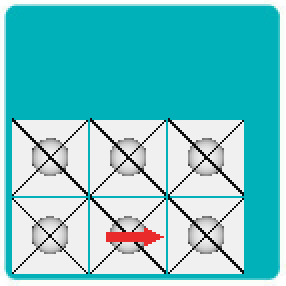
\includegraphics[width=.7\linewidth]{figures/F3-7.png}
  \caption{button layout: \papertitle 5}
  \label{fig:f3g}
  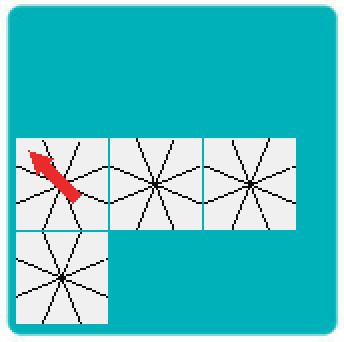
\includegraphics[width=.7\linewidth]{figures/F3-8.png}
  \caption{button layout: \papertitle 8}
  \label{fig:f3h}
\end{subfigure}
\caption{Sample layout of User Study for designing \papertitle (a),(b) button shape test layout. Each layout contains 18 buttons. (c), (d) button size test layout. (e), (f) swipe per button test layout. Each button is 10 mm per side. (e) is 7 swipe button with a highlight circle to instruct user to tap on that button (f) is 10 swipe button with an arrow instruct user to perform left swipe.  (g), (h) button layout test layout. Each layout is confined in a 15 x 25 mm space}
\label{fig:f3}
\end{figure*}

Figure 2 shows some examples of different keyboard layouts that we have tested during our user study. In this test, a single random button will light up in red. A circle in a button can either be lit up red or an arrow will light up. If a circle in the button is highlighted, the user simply needs to tap on the corresponding button. On the other hand, if a highlighted arrow appears, then the user needs to swipe on that button toward the direction indicted by the arrow. For this swipe motion, the finger must press and start from the button with the highlighted arrow. After initiating the swipe the user can let go of the screen anywhere as long as the finger motion follows the direction the highlighted arrow pointing towards.

After the user finished tapping or swiping on a button, a new random button will light up. The user gains a point every time the user taps or swipes on the correct button and towards the correct direction. In case of mistakes, such as missing the highlighted button or not swiping towards the correct direction, would produce a red flash on the screen. The user will not gain any point for any misses. The user must get as many points as possible within a 60 second time frame. After the timer is up, the screen will display the number of hits, the number of total taps and swipes, and the percentage of hits over the total number of taps and swipes.

In this user study for designing \papertitle, we have conducted this test with 12 users with ages ranging from 19 to 35 (7 male and 5 female).

\subsection{Button Shape}
We have decided to make the keyboard buttons square shaped for 3 reasons, inspired by the consideration of I Scott MacKenzie \cite{opti}:
\begin{itemize}
\item[1.]Square or rectangular shaped buttons can be tightly packed together in a grid formation without leaving empty gaps between each button (dead space)
\item[2.]Square shaped buttons are better for touch accuracy compared to rectangular shaped buttons
\item[3.]Square shaped buttons make every swipe direction angles equal. For example, if the aspect ratio for horizontal/vertical were 2, then it would be easier to swipe horizontally than vertically. If, on the other hand, the buttons are square, then swiping horizontally or vertically will have equal accuracy.
\end{itemize}

The second statement above is demonstrated in Lee’s work \cite{performance-of-soft-button}. He showed that square-like buttons (wider button) are more preferable than rectangle-like buttons (narrow buttons). To further study the effect of the role of aspect ratio, we have conducted a user study of button shape on buttons with different aspect ratio but with the same size. Users were asked to tap on a random highlighted button continuously. Figure 2(a) and (b) show the sample test layout.

The result in Figure 3 shows that both error rate and tapping speed will worsen for an aspect ratio different from 1. This suggests that a keyboard design with buttons close to being square shaped is preferred for high speed and low error text entry.

\begin{figure}
  \begin{subfigure}{1\columnwidth}
  \centering
  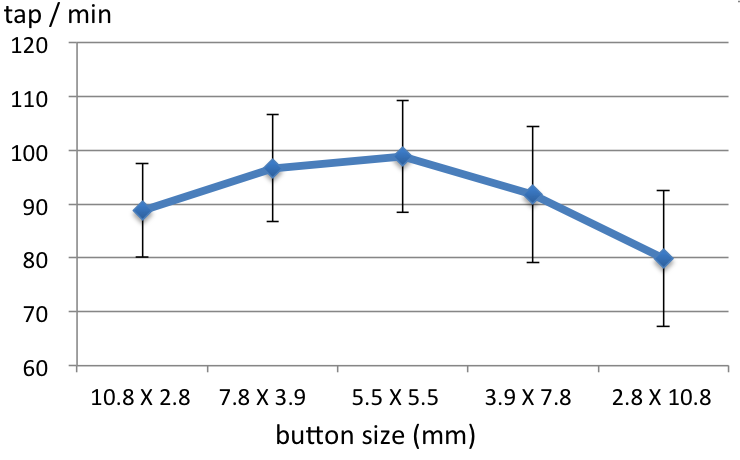
\includegraphics[width=.8\columnwidth]{figures/F4-1.png}
  \caption{}
  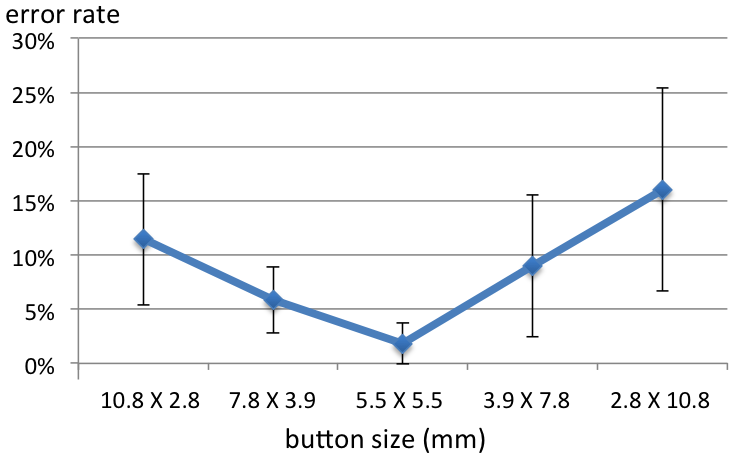
\includegraphics[width=.8\columnwidth]{figures/F4-2.png}
  \caption{}
  \label{fig:f4}
  \end{subfigure}
  \caption{Button shape test result. (a) Tap speed of 12 users (c) Error rate}
\end{figure}

\subsection{Button Size and Swipe per Button}
The size of the keyboard and the number of characters are two constrains that connect the button size and swipes per button. Our final goal was to put 26 possible entries (characters in the alphabet) onto the smartwatch keyboard. That means that if we had a keyboard that heavily relied on using swipe motions instead of using tap motions to select entries on a button, we could have made each button bigger. Therefore, we needed to consider at the same time these two correlated parameters: the number of possible swipe directions per button and the button size. Even if they are dependent on each other, we still had to test them individually in separate experiments to further understand the importance of both parameters.

For the experiment involving button sizes, we created different keyboard designs, each with differently sized buttons. On one hand, having bigger buttons meant that the users had an easier time pressing each of them accurately, but it also meant that we would not be able to fit many buttons on the smartwatch screen. On the other hand, we would be able to place more buttons on the screen if the buttons are small, but it would have meant that the users would have difficulty pressing each button accurately. During the experiment, users were asked to tap on differently sized square buttons similar to the previous tests. We evaluated them on how many correct button presses they made for each of the button sizes. After testing, we asked the user which button size they had trouble tapping on correctly. The results are shown in Figure 4.

\begin{figure}
  \begin{subfigure}{1\columnwidth}
  \centering
  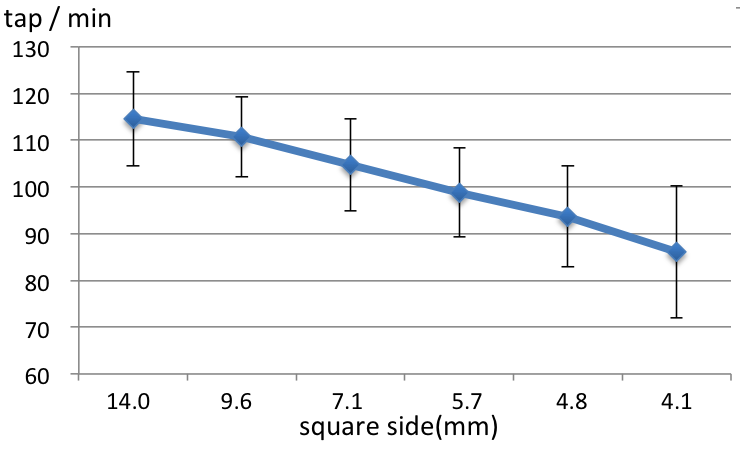
\includegraphics[width=.8\columnwidth]{figures/F5-1.png}
  \caption{}
  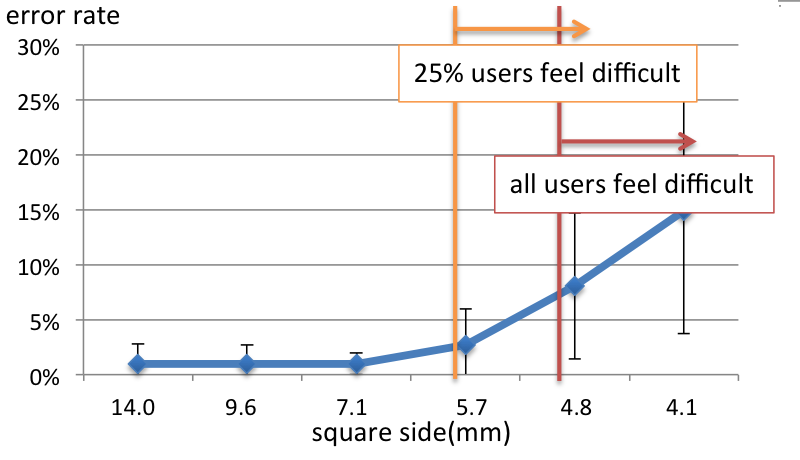
\includegraphics[width=.8\columnwidth]{figures/F5-2.png}
  \caption{}
  \label{fig:f5}
  \end{subfigure}
  \caption{Result of button size test. (a) Tap speed (b) Error rate}
\end{figure}

The results show that the speed decreases steadily as we make the button size smaller. The error rate rises dramatically for button size smaller than 5.7mm x 5.7mm. All the users felt that it was difficult to tap on the correct button with button size smaller than 4.8mm x 4.8mm. About 25\% of the users felt that tapping on 5.7mm x 5.7mm buttons was difficult. It suggests making keyboard buttons at least 5.7mm x 5.7mm large.

Then we designed a test to investigate the accuracy of swipe motions. In this test, a large button is divided into different angle sections. An arrow will randomly light up red and the user is asked to swipe towards the direction the arrow is pointing towards from the center of the button. Different button designs may allow different amounts of swipe directions. The number of swipe directions determines the number of directions the arrow can point. For example, if a button design has 4 swipe directions, it means that the arrow can end up pointing at 4 possible directions: up, down, left, and right. Figure 2 (f) shows a button with 10 swipe directions, meaning the arrow can point towards any of the 10 directions (mixture of left, right, and diagonal swipes). A button with small number of swipe directions would be easier to swipe in the correct direction than ones with a large number. This is because users need to be more precise with the angle of the swipe he or she makes with buttons with more swipe directions. In other words, a button 4 swipe direction has more tolerance in swipe angle than ones with 10 swipe directions. Clearly, we do not want to have too many swipe directions per button, or else the keyboard will be difficult to use.

Users were asked to swipe to towards a random chosen direction on a 10 x 10 mm button. Since we consider both vertical and horizontal symmetry, only even swipe numbers are taken into account. In addition, there are many works that combine tap with swipe for text entry buttons. Therefore, we also consider every even swipe with an additional tap as a candidate \papertitle\ button. After this test, we also asked the user to choose buttons that are hard to follow correctly. Note that the odd number swipe represents its lower even number swipe plus one tap. The sample layout is in Figure 2(e), (f). The results of the experiment are shown in Figure 5.

Figure 5(a) shows that the swipe speed is about 90 swipes per minute on average, and the swipe speed is almost independent to swipes per button. But the error rate and user experience is highly correlated with the number of swipes per button. The error rate rises when the number of swipes per button is larger than 8 swipes. Notice that even though the error rate is low for 6 swipes, 17\% of the users felt that it was difficult to swipe correctly with this number of swipe directions. Moreover, the layout with tap and swipe has higher accuracy (???) than the group with swipe only. It suggests that the combination of 2 different types of movements (tap and swipe) might increase the possibility of making errors. This inconsistency between tap and swipe is also reported by 25\% of users. 

\begin{figure}
  \begin{subfigure}{1\columnwidth}
  \centering
  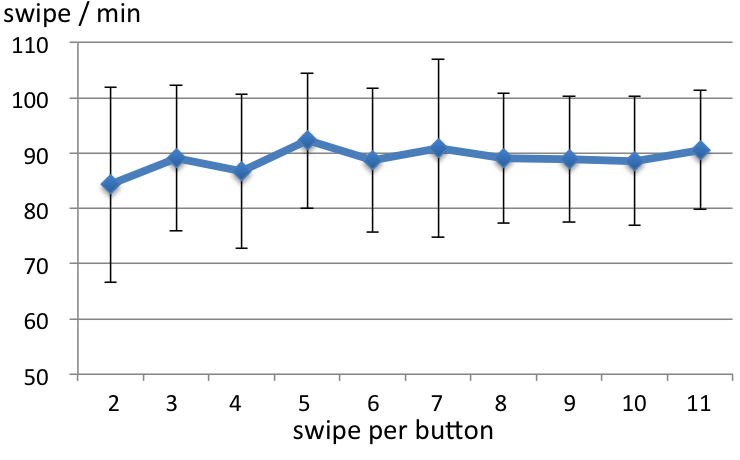
\includegraphics[width=.8\columnwidth]{figures/F6-1.png}
  \caption{}
  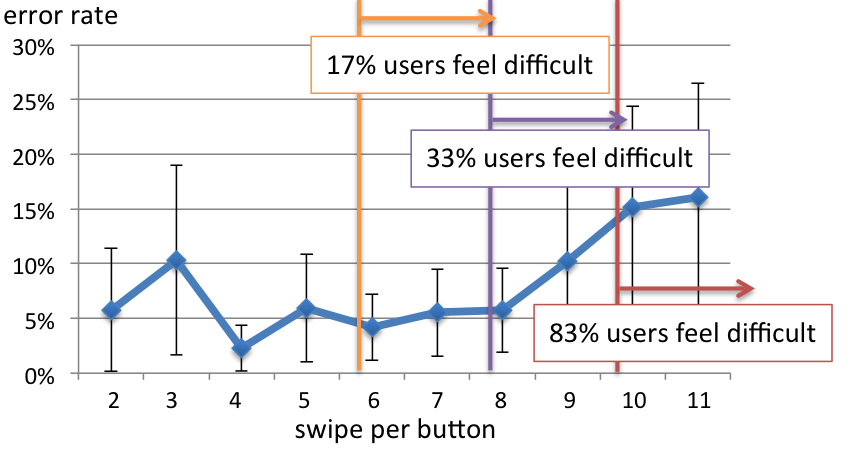
\includegraphics[width=.8\columnwidth]{figures/F6-2.png}
  \caption{}
  \label{fig:f6}
  \end{subfigure}
  \caption{Result of swipe per button test. (a) Swipe speed (b) Error rate}
\end{figure}

\subsection{Button Layout}

Based on the keyboard space and a minimum of 26 entries, we can arrange many possible layouts for each swipe number of \papertitle. Each swipe number of \papertitle\ has one layout with maximum button size. The layout choices of different swipe numbers \papertitle\ are shown in Table 1.

\begin{table}[t]
  \begin{center}
  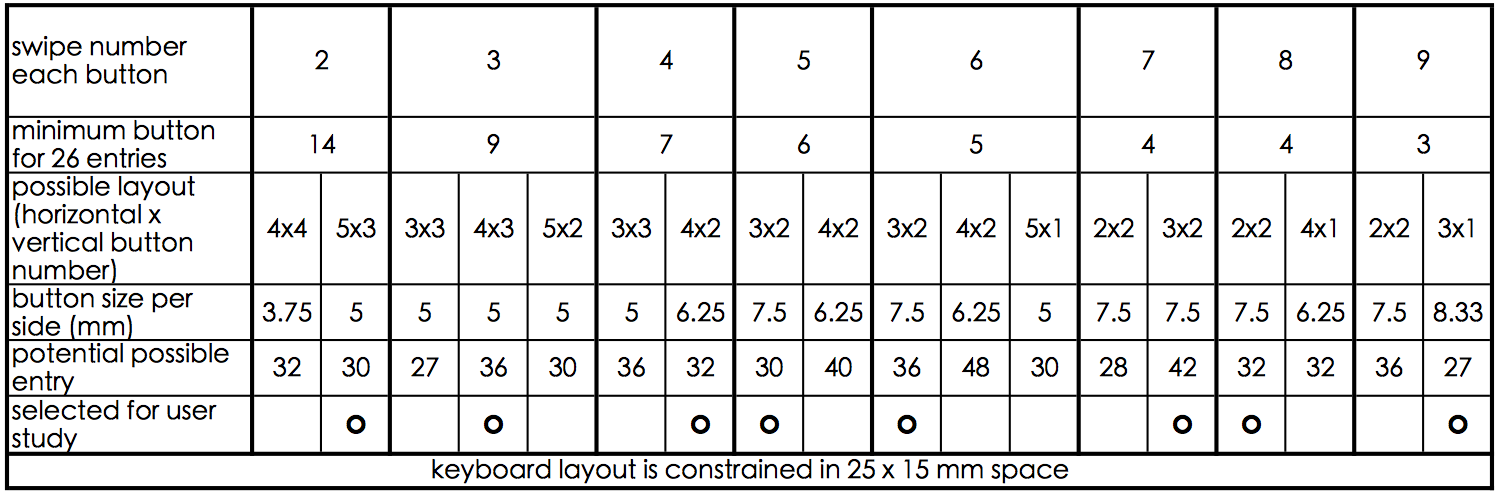
\includegraphics[width=1\columnwidth]{figures/T1.png}
  \caption[Table 1]{Layout decisions for different swipe number \papertitle. We select the layout with a largest square button size of a specific swipe number. If sizes are the same between many layouts, we then select the layout with the maximum number of potential entries.}
  \label{tab:t1}
  \end{center}
\end{table}

To investigate the influence of different swipe number layouts, we ran a user study as a continuation of our previous studies. Users were asked to swipe or tap at a random selected button and direction from 26 possible entries of 8 different types of \papertitle\ layouts. After that, users were asked to answer a questionnaire about the difficulty rating of each layout and voted for a preferred layout. Figure 6 shows the test results.

The small button size in \papertitle\ 2 and \papertitle\ 4 layouts were the worst in terms of input speed and error rate. This result is consistent with our button size user study: the error rate increases drastically if the button size is smaller than 5.7mm x 5.7mm. The large button size group also suffers a slight speed drop and error rate increase due to many possible swipe directions for each button. Although the \papertitle\ 4 and 5 layouts are the best for error rate and speed, these layouts have a nearly identical error rate and speed of \papertitle\ 6 and 7 layouts. On the other hand, user ratings paint a clearer picture. Figure 6 (c) shows that \papertitle\ 4 and 5 layouts outperform other candidates in difficulty rating and preference. Therefore, we have selected \papertitle\ 4 and 5 layouts to represent the official \papertitle\ layouts for our smartwatch text entry solution.

\subsection{Character Arrangement}
The last piece of the puzzle in designing SwipeKey is figuring out how to arrange the 26 characters in the alphabet. We considered an alphabetically ordered character layout because it is a common keyboard character layout \cite{text-entry-theory}. Secondly, there is evidence that experts typing on a keyboard with alphabetical layout perform just as well as experts typing on a QWERTY layout keyboard \cite{text-entry-theory,abc-not-matter}. Thirdly, \papertitle\ is a different type of keyboard. We did not have a proven way of transforming common keyboard layouts, such as QWERTY and Dvorak, and applying them to SwipeKey.

\begin{figure}
  \begin{subfigure}{1\columnwidth}
  \centering
  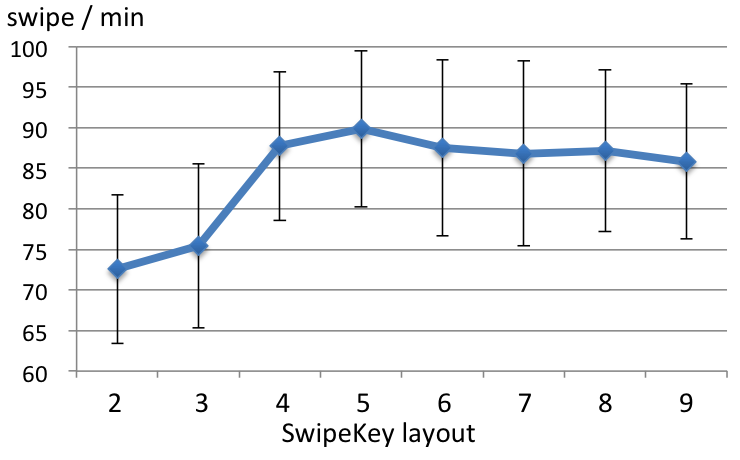
\includegraphics[width=.8\columnwidth]{figures/F7-1.png}
  \caption{}
  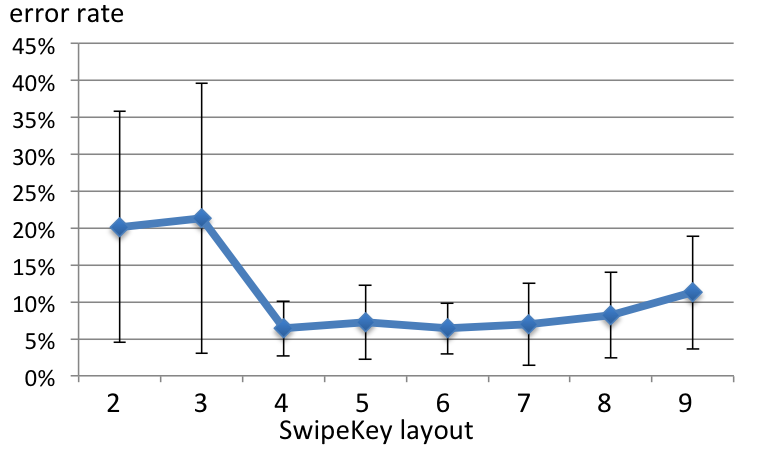
\includegraphics[width=.8\columnwidth]{figures/F7-2.png}
  \caption{}
  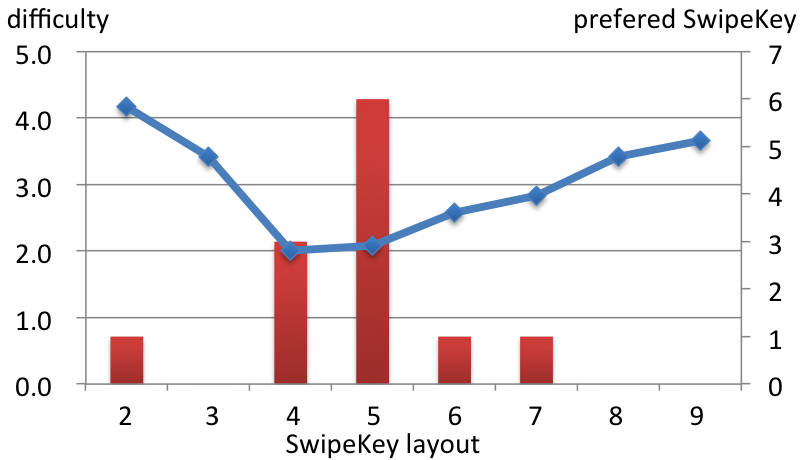
\includegraphics[width=.8\columnwidth]{figures/F7-3.png}
  \caption{}
  \label{fig:f7}
  \end{subfigure}
  \caption{Result of button layout test. (a) Test speed (b) Test error rate (c) Button layout test difficulty rating and participants preferred button layout}
\end{figure}
\section{User Study: \papertitle\ prototype implemented on an Android Smartwatch}

To test the performance of \papertitle, we have implemented \papertitle\ 4 and \papertitle\ 5 on the Sony SmartWatch 3 running Android 4.4. We have also implemented Autodesk Research's Swipeboard on our system for comparison purpose since it performs well on smartwatches compared to other existing keyboards. Swipeboard's performance is compatible or better than that of Zoomboard \cite{swipeboard}. However, Swipeboard has a QWERTY based keyboard layout. In order to separate the factor of keyboard layout from character arrangement, we have also implemented a Swipeboard-like keyboard in alphabetical order. To make the keyboard consistent, we have removed the button with 4 characters: r, t, y, u and allowed buttons to have only 3 characters each. For all of the keyboards we have implemented, the users can delete characters (backspace) or enter a space (spacebar) in a consistent way. To delete a character, users can swipe left on the text entry space. To enter a space, the users can swipe right on the text entry space. Figure 7 shows all the keyboard designs.

\begin{figure*}
\begin{subfigure}{.24\textwidth}
  \centering
  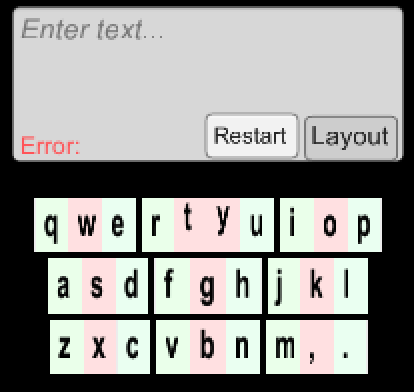
\includegraphics[width=.8\linewidth]{figures/F8-1.png}
  \caption{}
  \label{fig:f8a}
\end{subfigure}%
\begin{subfigure}{.24\textwidth}
  \centering
  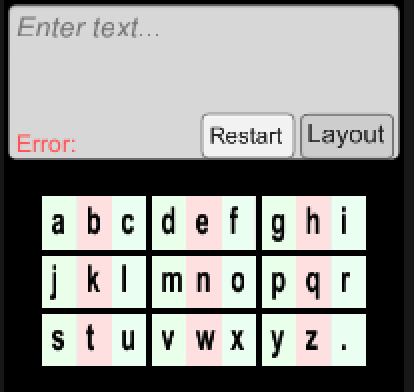
\includegraphics[width=.8\linewidth]{figures/F8-2.png}
  \caption{}
  \label{fig:f8b}
\end{subfigure}
\begin{subfigure}{.24\textwidth}
  \centering
  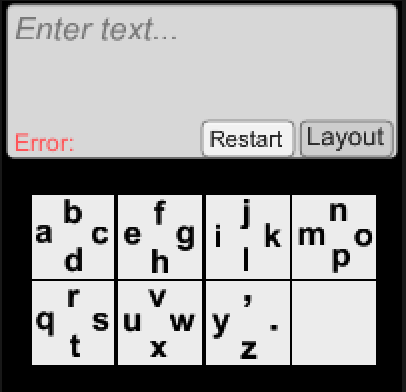
\includegraphics[width=.8\linewidth]{figures/F8-3.png}
  \caption{}
  \label{fig:f8c}
\end{subfigure}
\begin{subfigure}{.24\textwidth}
  \centering
  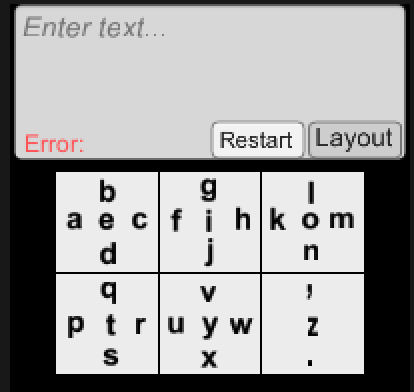
\includegraphics[width=.8\linewidth]{figures/F8-4.png}
  \caption{}
  \label{fig:f8d}
\end{subfigure}
\caption{Keyboard layout on smartwatch (a) Swipeboard (b) Swipeboard (Alphabetical) (c) \papertitle 4 (d) \papertitle 5}
\label{fig:f8}
\end{figure*}

\subsection{Participants}
We have recruited 12 participants for this test. Of these 12 participants, 7 were male and 5 were female. The average age is 24 years old. 9 participants stated that they could perform blind-typing on a PC keyboard. 10 participants were right-handed. All participants own touchscreen smartphones and 5 of them have used a smartwatch before.

\subsection{Task}
Participants were given a total of 2 minutes to get familiar with each type of keyboard before the test. They were told to use their index finger of their dominant hand to enter text. Each participant had to run 6 task blocks per keyboard, where the users were asked to type out 5 phrases per task block. In other words, they were asked to type out 30 phrases for each keyboard layout in a predetermined counter-balanced order. All in all, each user saw a total of 120 different phrases throughout the test. These test phrases were drawn randomly from the 500-phrase corpus compiled by MacKenzie and Soukoreff \cite{phrase-set}. A big screen in front of the user was used to display a phrase and the user then entered the displayed text on the smartwatch keyboard. The screen displayed the current phrase the user was supposed to be typing. The screen switched to showing the next phrase only when the participant finished typing out the current phrase. The reason for displaying each phrase on the screen rather than asking users to memorize each phrase was to avoid memorability bias. In all of the trials, we have instructed the participants to correct their mistakes as they were typing on the keyboard. They can swipe left on the text entry space to delete a character they have mistyped and then retype the correct character. However, if they fail to notice a mistake and only realize it after typing several more characters, they would then ignore the mistake and continue typing normally. At the end of the test, participants completed a short questionnaire and a short interview.

\subsection{Result and Discussion}

\subsubsection{Text Entry Speed}

\begin{figure}[t]
  \begin{subfigure}{1\columnwidth}
  \centering
  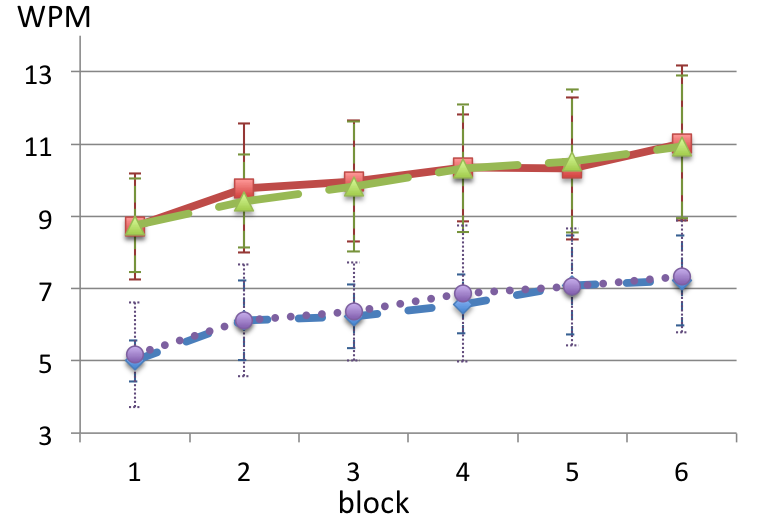
\includegraphics[width=.8\columnwidth]{figures/F9-1.png}
  \caption{}
  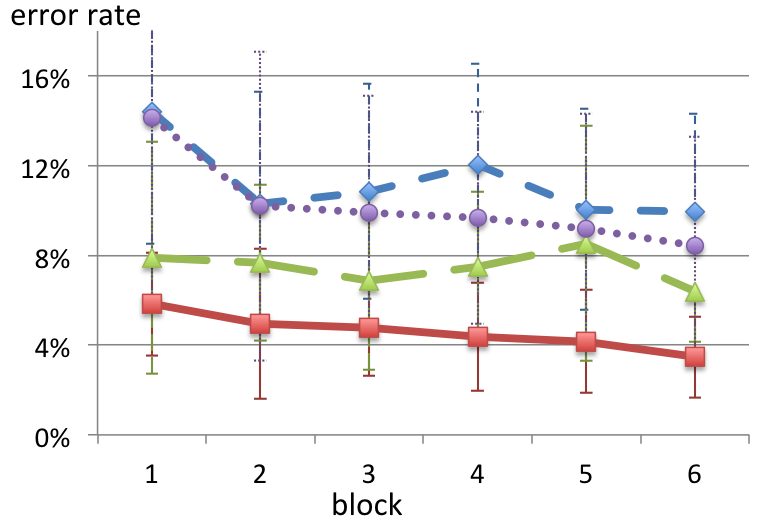
\includegraphics[width=.8\columnwidth]{figures/F9-2.png}
  \caption{}
  \label{fig:f9}
  \end{subfigure}
  \caption{ Quantitative results of user study for \papertitle verification (a) WPM (b) error rate}
\end{figure}

Figure 8 (a) shows the aggregated WPM results of the 12 users (including error correction time). Swipeboard (QWERTY layout) had 5.0 WPM in the first block. After more than half an hour of training, the typing speed rose to 7.3 WPM in the last block. The WPM curve of Swipeboard (QWERTY) is slightly lower and almost overlaps with that of Swipeboard (alphabetical), with a 5.3 WPM in the first block and 7.4 WPM in the end. The result suggests that the QWERTY keyboard layout does not help the users type faster than users who use an alphabetical keyboard layout. It also supports our design decision of using alphabetical grouping. Two of our users mentioned that the feeling of typing on Swipeboard (QWERTY) is totally different from typing on a mechanical keyboard, despite the fact that both users are capable of blind-typing. It is hard for them to transfer their muscle memory of using a mechanical QWERTY layout to the Swipeboard input method even if it is based on QWERTY. This might be a possible reason why QWERTY is not particularly helpful for character location memorization.

The WPM of \papertitle\ 4 and \papertitle\ 5 are 8.7 and 8.8 respectively in the first block, and 11 and 10.9 respectively in the last block. \papertitle\ 4 and \papertitle\ 5 are comparable in terms of speed even after the users got some practice. The WPM of \papertitle\ group is much higher than that of the Swipeboard group. There is a significant performance difference among all the test data (F(1,262)=283.4, p << .001). The initial speed of the \papertitle\ group is even faster than that of the trained Swipeboard group. It shows that the speed gap between \papertitle\ and Swipeboard is at about 4 WPM across all tests. This might imply a non-converging typing speed between these 2 groups even after long-term training. The superiority of \papertitle\ in speed is due to the second design requirement. \papertitle\ is expected to have a shorter reaction time for each character. It takes 1 swipe for each character while Swipeboard requires 2.

\subsubsection{Error Rate}
In Figure 8 (b), the error rate in the beginning is comparable between Swipeboard (QWERTY) and Swipeboard (alphabetical). Though, after a short training session, Swipeboard (alphabetical) shows a slightly lower error rate in the last 3 blocks (F(1,64) = 2.17, p = 0.14). Six users reported that they made more mistakes when they tried to type out the 't' and 'y' characters located on the 'rtyu' button of the Swipeboard (QWERTY). One user found the 'rtyu' button inconsistent and confusing because that button consisted of 4 characters while the other 8 buttons in the layout consisted of only 3. 

The average error rate for the Swipeboard group (10.9\%) is about half of the error rate for the \papertitle\ group (5.8\%) across all tests (F(1,262)=71.9, p << .001). This could be explained by 2 factors. Firstly, Swipeboard users needed to make 2 swipes in order to type a single character, which increased the error rate due to the extra swipe. \papertitle\ users needed to make only 1 swipe per character. Secondly, the inconsistent swipe directions in the first (8 directional swipes + 1 tap) and the second layer (2 directional swipes + 1 tap or 4 directional swipes) introduce a higher error rate. Users also reported that \papertitle\ is more intuitive to use.

For in-group comparison of \papertitle, \papertitle\ 4 had a significantly lower error rate (4.4\% on average, 3.4\% for the last block) compared to \papertitle\ 5 (7.4\% on average, 6.3\% for the last block) (F(1,130)=26.4, p < .001). We already noticed this phenomenon in our previous user study when designing \papertitle, and we believe that it is caused by inconsistent design and combination of 2 different types of movement: tap and swipe. Some participants mentioned that their tap was accepted as a swipe and that they could not distinguish which is more likely to happen. 

\subsubsection{User Survey}

\begin{figure}[h]
  \begin{subfigure}{1\columnwidth}
  \centering
  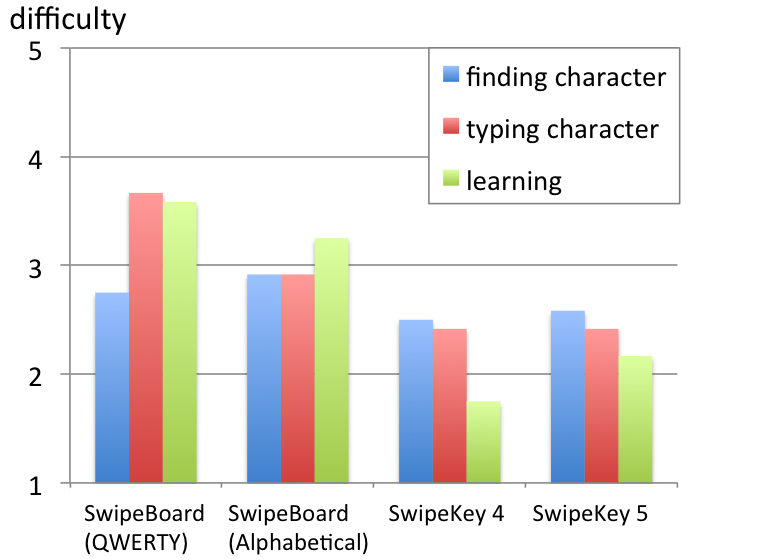
\includegraphics[width=.8\columnwidth]{figures/F10-1.png}
  \caption{}
  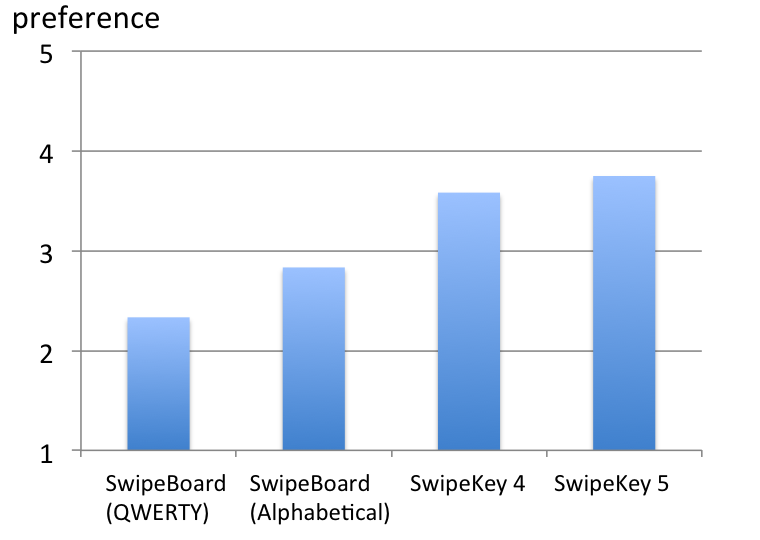
\includegraphics[width=.8\columnwidth]{figures/F10-2.png}
  \caption{}
  \label{fig:f10}
  \end{subfigure}
  \caption{ (a) User rating of difficulty on a 5-point Likert scale for finding a character, typing a located character, and learning how to use different keyboards. (b) User preference of different keyboards}
\end{figure}

We summarize 3 different kinds of difficulty rating of keyboard layouts in Figure 9 (a). There is no significant difference in finding a character between Swipeboard (QWERTY) and Swipeboard (alphabetical). However, there are 3 users who said that they found it more difficult to find characters on the alphabetically ordered keyboard. Their difficulty rating for finding characters on the alphabetically ordered keyboard is much higher than that of other users (average 3.9 point of the 3 users compared with 2.7 point of 12 users). The rest of the users did not find the QWERTY layout more helpful.

Typing characters on Swipeboard (QWERTY) is the most difficult. This is revealed in our interview with users. Our users mentioned that “It is hard to swipe 'r' and 't', and it continuously enters the wrong character“, “Sometimes, my swipe on the first layer keeps entering the wrong group of characters”, or “The 't' and 'y' are hard to type”. 
Considering the difficulty of learning for each keyboard, we see that \papertitle\ is easier to learn compared to Swipeboard (F(1,42)=21.1,  p=0.004). One of the participants said that it took him a while to get accustomed to Swipeboard, but he could use \papertitle\ immediately. However, those who had difficulty in finding characters do feel that there is a high learning curve for \papertitle (average 3.5 compared with total average 2.0).

In Figure 9 (b), the preference for \papertitle\ in a 5-point Likert scale is higher than that of Swipeboard (F(1,42)=17.8,  p=0.013). Most of the users said that they prefer SwipeKey because it is intuitive and easier to use compared to Swipeboard. However, there is still one participant that prefers Swipeboard (QWERTY) due to the QWERTY layout, despite the fact that both speed and error rate of that particular participant are better with \papertitle.

\section{Limitation and Conclusion}
In this work, we have focused on creating a one swipe or one tap keyboard for smartwatches. We have first discussed the 3 qualities of optimized keyboards. These requirements outline the design for \papertitle, and allowed us to conduct a series of user studies to narrow down the numbers of possible design options. We have implemented \papertitle\ 4 and \papertitle\ 5, both optimized for WPM, error rate, rating of difficulty and user preference. The result of \papertitle\ shows a 55\% improvement in WPM and a 44\% decrease in error rate compared to Swipeboard. We have discovered that the QWERTY keyboard layout does not provide significant advantages to small swipe-based keyboards according our experiment. This knowledge could be helpful for future keyboard designs on small devices since keyboard designers are not forced to distort their keyboard designs to accommodate the QWERTY layout.

There is an important design principle that emerges from our user study. A consistent design is crucial for intuitive, easy to use, and low error rate keyboard layouts.

We have focused our work on keyboard design for smartwatches. As suggested in the work of Luis etals. \cite{text-entry-on-small-qwerty}, designing a suitable keyboard depends on the screen size. For a smaller keyboard size, we may find that an even higher swipe direction number \papertitle\ such as \papertitle\ 6 or even \papertitle\ 9 may outperform \papertitle\ 4 or 5. This is because as the keyboard space becomes smaller, the button size will shrink accordingly, and eventually the size of a button would become smaller than the acceptable minimum size, leading to a drastic increase in input errors. Note that the error rate increases more slowly when increasing the number of swipe directions compared to shrinking the button size below a certain size limit.

Modern soft keyboards use word prediction and auto-correction to improve performance. Although we did not take this effect into consideration in this paper, it is possible to further improve \papertitle\ by integrating these features in future works.

We believe that our work provides a well-designed keyboard for smartwatches that enables intuitive, fast, and low error text entry. Smartwatch manufacturers can implement \papertitle\ on smartwatches, along with other input methods, such as voice input, to provide more choices for the users. Furthermore, this work provides a new understanding of swipe resolution and character arrangement on small devices. This information could be helpful for future researchers.


% \section{Introduction}

% This format is to be used for submissions that are published in the
% conference proceedings. We wish to give this volume a consistent,
% high-quality appearance. We therefore ask that authors follow some
% simple guidelines. You should format your paper exactly like this
% document. The easiest way to do this is to replace the content with
% your own material.  This document describes how to prepare your
% submissions using \LaTeX.

% \section{Page Size and Columns}
% On each page your material should fit within a rectangle of 7 $\times$
% 9.25 inches (18 $\times$ 23.5 cm), centered on a US Letter page (8.5
% $\times$ 11 inches), beginning 0.75 inches (1.9 cm) from the top of
% the page, with a 0.33 inches (0.85 cm) space between two 3.3 inches
% (8.4 cm) columns. Right margins should be justified, not
% ragged. Please be sure your document and PDF are US letter and not A4.

% \section{Typeset Text}
% The styles contained in this document have been modified from the
% default styles to reflect ACM formatting conventions. For example,
% content paragraphs like this one are formatted using the Normal style.

% \LaTeX\ sometimes will create overfull lines that extend into columns.
% To attempt to combat this, the \texttt{.cls} file has a command,
% \texttt{{\textbackslash}sloppy}, that essentially asks \LaTeX\ to
% prefer underfull lines with extra whitespace.  For more details on
% this, and info on how to control it more finely, check out
% {\url{http://www.economics.utoronto.ca/osborne/latex/PMAKEUP.HTM}}.

% \subsection{Title and Authors}

% Your paper's title, authors and affiliations should run across the
% full width of the page in a single column 17.8 cm (7 in.) wide.  The
% title should be in Helvetica or Arial 18-point bold.  Authors' names
% should be in Times New Roman or Times Roman 12-point bold, and
% affiliations in 12-point regular.  

% See \texttt{{\textbackslash}author} section of this template for
% instructions on how to format the authors. For more than three
% authors, you may have to place some address information in a footnote,
% or in a named section at the end of your paper. Leave one 10-point
% line of white space below the last line of affiliations.

% \subsection{Abstract and Keywords}

% Every submission should begin with an abstract of about 150 words,
% followed by a set of Author Keywords and ACM Classification
% Keywords. The abstract and keywords should be placed in the left
% column of the first page under the left half of the title. The
% abstract should be a concise statement of the problem, approach, and
% conclusions of the work described. It should clearly state the paper's
% contribution to the field of HCI\@.

% \subsection{Normal or Body Text}

% Please use a 10-point Times New Roman or Times Roman font or, if this
% is unavailable, another proportional font with serifs, as close as
% possible in appearance to Times Roman 10-point. Other than Helvetica
% or Arial headings, please use sans-serif or non-proportional fonts
% only for special purposes, such as source code text.

% \subsection{First Page Copyright Notice}
% This template include a sample ACM copyright notice at the bottom of
% page 1, column 1.  Upon acceptance, you will be provided with the
% appropriate copyright statement and unique DOI string for publication.
% Accepted papers will be distributed in the conference
% publications. They will also be placed in the ACM Digital Library,
% where they will remain accessible to thousands of researchers and
% practitioners worldwide. See
% \url{http://acm.org/publications/policies/copyright_policy} for the
% ACM’s copyright and permissions policy.

% \subsection{Subsequent Pages}

% On pages beyond the first, start at the top of the page and continue
% in double-column format.  The two columns on the last page should be
% of equal length.

% \begin{figure}
% \centering
%   \includegraphics[width=0.9\columnwidth]{figures/sigchi-logo}
%   \caption{Insert a caption below each figure. Do not alter the
%     Caption style.}~\label{fig:figure1}
% \end{figure}

% \subsection{References and Citations}

% Use a numbered list of references at the end of the article, ordered
% alphabetically by last name of first author, and referenced by numbers
% in
% brackets~\cite{acm_categories,ethics,Klemmer:2002:WSC:503376.503378}.
% Your references should be published materials accessible to the
% public. Internal technical reports may be cited only if they are
% easily accessible (i.e., you provide the address for obtaining the
% report within your citation) and may be obtained by any reader for a
% nominal fee. Proprietary information may not be cited. Private
% communications should be acknowledged in the main text, not referenced
% (e.g., ``[Borriello, personal communication]'').

% References should be in ACM citation format:
% \url{http://acm.org/publications/submissions/latex_style}. This
% includes citations to internet
% resources~\cite{acm_categories,cavender:writing,CHINOSAUR:venue,psy:gangnam}
% according to ACM format, although it is often appropriate to include
% URLs directly in the text, as above.


% % Use a numbered list of references at the end of the article, ordered
% % alphabetically by first author, and referenced by numbers in
% % brackets~\cite{ethics, Klemmer:2002:WSC:503376.503378,
% %   Mather:2000:MUT, Zellweger:2001:FAO:504216.504224}. For papers from
% % conference proceedings, include the title of the paper and an
% % abbreviated name of the conference (e.g., for Interact 2003
% % proceedings, use \textit{Proc. Interact 2003}). Do not include the
% % location of the conference or the exact date; do include the page
% % numbers if available. See the examples of citations at the end of this
% % document. Within this template file, use the \texttt{References} style
% % for the text of your citation.

% % Your references should be published materials accessible to the
% % public.  Internal technical reports may be cited only if they are
% % easily accessible (i.e., you provide the address for obtaining the
% % report within your citation) and may be obtained by any reader for a
% % nominal fee.  Proprietary information may not be cited. Private
% % communications should be acknowledged in the main text, not referenced
% % (e.g., ``[Robertson, personal communication]'').

% \begin{table}
%   \centering
%   \begin{tabular}{r c c}
%     \toprule
%     & \multicolumn{2}{c}{\small{\textbf{Caption}}} \\
%     \cmidrule(r){2-3}
%     {\small\textbf{Objects}}
%     & {\small \textit{Pre-2002}}
%     & {\small \textit{Current}} \\
%     \midrule
%     Tables & Above & Below \\
%     Figures & Below & Below \\
%     \bottomrule
%   \end{tabular}
%   \caption{Table captions should be placed below the table. We
%     recommend table lines be 1 point, 25\% black. Minimize use of
%     unnecessary table lines.}~\label{tab:table1}
% \end{table}

% \section{Sections}

% The heading of a section should be in Helvetica or Arial 9-point bold,
% all in capitals. Sections should \textit{not} be numbered.

% \subsection{Subsections}

% Headings of subsections should be in Helvetica or Arial 9-point bold
% with initial letters capitalized.  For sub-sections and
% sub-subsections, a word like \emph{the} or \emph{of} is not
% capitalized unless it is the first word of the heading.

% \subsubsection{Sub-subsections}

% Headings for sub-subsections should be in Helvetica or Arial 9-point
% italic with initial letters capitalized.  Standard
% \texttt{{\textbackslash}section}, \texttt{{\textbackslash}subsection},
% and \texttt{{\textbackslash}subsubsection} commands will work fine in
% this template.

% \section{Figures/Captions}

% Place figures and tables at the top or bottom of the appropriate
% column or columns, on the same page as the relevant text (see
% Figure~\ref{fig:figure1}). A figure or table may extend across both
% columns to a maximum width of 17.78 cm (7 in.).

% \begin{figure*}
%   \centering
%   \includegraphics[width=2\columnwidth]{figures/map}
%   \caption{In this image, the map maximizes use of space. You can make
%     figures as wide as you need, up to a maximum of the full width of
%     both columns. Note that \LaTeX\ tends to render large figures on a
%     dedicated page. Image: \ccbynd~ayman on
%     Flickr.}~\label{fig:figure2}
% \end{figure*}

% Captions should be Times New Roman or Times Roman 9-point bold.  They
% should be numbered (e.g., ``Table~\ref{tab:table1}'' or
% ``Figure~\ref{fig:figure1}''), centered and placed beneath the figure
% or table.  Please note that the words ``Figure'' and ``Table'' should
% be spelled out (e.g., ``Figure'' rather than ``Fig.'') wherever they
% occur. Figures, like Figure~\ref{fig:figure2}, may span columns and
% all figures should also include alt text for improved accessibility.
% Papers and notes may use color figures, which are included in the page
% limit; the figures must be usable when printed in black-and-white in
% the proceedings.

% The paper may be accompanied by a short video figure up to five
% minutes in length. However, the paper should stand on its own without
% the video figure, as the video may not be available to everyone who
% reads the paper.  

% \subsection{Inserting Images}
% When possible, include a vector formatted graphic (i.e. PDF or EPS).
% When including bitmaps,  use an image editing tool to resize the image
% at the appropriate printing resolution (usually 300 dpi).

% \section{Language, Style and Content}

% The written and spoken language of SIGCHI is English. Spelling and
% punctuation may use any dialect of English (e.g., British, Canadian,
% US, etc.) provided this is done consis- tently. Hyphenation is
% optional. To ensure suitability for an international audience, please
% pay attention to the following:

% \begin{itemize}
% \item Write in a straightforward style.
% \item Try to avoid long or complex sentence structures.
% \item Briefly define or explain all technical terms that may be
%   unfamiliar to readers.
% \item Explain all acronyms the first time they are used in your
%   text---e.g., ``Digital Signal Processing (DSP)''.
% \item Explain local references (e.g., not everyone knows all city
%   names in a particular country).
% \item Explain ``insider'' comments. Ensure that your whole audience
%   understands any reference whose meaning you do not describe (e.g.,
%   do not assume that everyone has used a Macintosh or a particular
%   application).
% \item Explain colloquial language and puns. Understanding phrases like
%   ``red herring'' may require a local knowledge of English.  Humor and
%   irony are difficult to translate.
% \item Use unambiguous forms for culturally localized concepts, such as
%   times, dates, currencies, and numbers (e.g., ``1--5--97'' or
%   ``5/1/97'' may mean 5 January or 1 May, and ``seven o'clock'' may
%   mean 7:00 am or 19:00). For currencies, indicate equivalences:
%   ``Participants were paid {\fontfamily{txr}\selectfont \textwon}
%   25,000, or roughly US \$22.''
% \item Be careful with the use of gender-specific pronouns (he, she)
%   and other gendered words (chairman, manpower, man-months). Use
%   inclusive language that is gender-neutral (e.g., she or he, they,
%   s/he, chair, staff, staff-hours, person-years). See the
%   \textit{Guidelines for Bias-Free Writing} for further advice and
%   examples regarding gender and other personal
%   attributes~\cite{Schwartz:1995:GBF}. Be particularly aware of
%   considerations around writing about people with disabilities.
% \item If possible, use the full (extended) alphabetic character set
%   for names of persons, institutions, and places (e.g.,
%   Gr{\o}nb{\ae}k, Lafreni\'ere, S\'anchez, Nguy\~{\^{e}}n,
%   Universit{\"a}t, Wei{\ss}enbach, Z{\"u}llighoven, \r{A}rhus, etc.).
%   These characters are already included in most versions and variants
%   of Times, Helvetica, and Arial fonts.
% \end{itemize}

% \section{Accessibility}
% The Executive Council of SIGCHI has committed to making SIGCHI
% conferences more inclusive for researchers, practitioners, and
% educators with disabilities. As a part of this goal, the all authors
% are asked to work on improving the accessibility of their
% submissions. Specifically, we encourage authors to carry out the
% following five steps:
% \begin{enumerate}
% \item Add alternative text to all figures
% \item Mark table headings
% \item Add tags to the PDF
% \item Verify the default language
% \item Set the tab order to ``Use Document Structure''
% \end{enumerate}
% For more information and links to instructions and resources, please
% see: \url{http://chi2016.acm.org/accessibility}.  The
% \texttt{{\textbackslash}hyperref} package allows you to create well tagged PDF files,
% please see the preamble of this template for an example.

% \section{Page Numbering, Headers and Footers}
% Your final submission should not contain footer or header information
% at the top or bottom of each page. Specifically, your final submission
% should not include page numbers. Initial submissions may include page
% numbers, but these must be removed for camera-ready. Page numbers will
% be added to the PDF when the proceedings are assembled.

% \section{Producing and Testing PDF Files}

% We recommend that you produce a PDF version of your submission well
% before the final deadline.  Your PDF file must be ACM DL
% Compliant. The requirements for an ACM Compliant PDF are available at:
% {\url{http://www.sheridanprinting.com/typedept/ACM-distilling-settings.htm}}.

% Test your PDF file by viewing or printing it with the same software we
% will use when we receive it, Adobe Acrobat Reader Version 10. This is
% widely available at no cost. Note that most
% reviewers will use a North American/European version of Acrobat
% reader, so please check your PDF accordingly.

% When creating your PDF from Word, ensure that you generate a tagged
% PDF from improved accessibility. This can be done by using the Adobe
% PDF add-in, also called PDFMaker. Select Acrobat | Preferences from
% the ribbon and ensure that ``Enable Accessibility and Reflow with
% tagged Adobe PDF'' is selected. You can then generate a tagged PDF by
% selecting ``Create PDF'' from the Acrobat ribbon.

% \section{Conclusion}

% It is important that you write for the SIGCHI audience. Please read
% previous years’ proceedings to understand the writing style and
% conventions that successful authors have used. It is particularly
% important that you state clearly what you have done, not merely what
% you plan to do, and explain how your work is different from previously
% published work, i.e., the unique contribution that your work makes to
% the field. Please consider what the reader will learn from your
% submission, and how they will find your work useful. If you write with
% these questions in mind, your work is more likely to be successful,
% both in being accepted into the conference, and in influencing the
% work of our field.

% \section{Acknowledgments}

% Sample text: We thank all the volunteers, and all publications support
% and staff, who wrote and provided helpful comments on previous
% versions of this document. Authors 1, 2, and 3 gratefully acknowledge
% the grant from NSF (\#1234--2012--ABC). \textit{This whole paragraph is
%   just an example.}

% Balancing columns in a ref list is a bit of a pain because you
% either use a hack like flushend or balance, or manually insert
% a column break.  http://www.tex.ac.uk/cgi-bin/texfaq2html?label=balance
% multicols doesn't work because we're already in two-column mode,
% and flushend isn't awesome, so I choose balance.  See this
% for more info: http://cs.brown.edu/system/software/latex/doc/balance.pdf
%
% Note that in a perfect world balance wants to be in the first
% column of the last page.
%
% If balance doesn't work for you, you can remove that and
% hard-code a column break into the bbl file right before you
% submit:
%
% http://stackoverflow.com/questions/2149854/how-to-manually-equalize-columns-
% in-an-ieee-paper-if-using-bibtex
%
% Or, just remove \balance and give up on balancing the last page.
%
% \balance{}

% \section{References Format}
% Your references should be published materials accessible to the
% public. Internal technical reports may be cited only if they are
% easily accessible (i.e., you provide the address for obtaining the
% report within your citation) and may be obtained by any reader for a
% nominal fee. Proprietary information may not be cited. Private
% communications should be acknowledged in the main text, not referenced
% (e.g., ``[Golovchinsky, personal communication]'').

% Use a numbered list of references at the end of the article, ordered
% alphabetically by first author, and referenced by numbers in
% brackets~\cite{ethics,Klemmer:2002:WSC:503376.503378}. For papers from
% conference proceedings, include the title of the paper and an
% abbreviated name of the conference (e.g., for Interact 2003
% proceedings, use Proc.\ Interact 2003). Do not include the location of
% the conference or the exact date; do include the page numbers if
% available. See the examples of citations at the end of this document
% and in the accompanying \texttt{BibTeX} document.

% References \textit{must be the same font size as other body
%   text}. References should be in alphabetical order by last name of
% first author. Example reference formatting for individual journal
% articles~\cite{ethics}, articles in conference
% proceedings~\cite{Klemmer:2002:WSC:503376.503378},
% books~\cite{Schwartz:1995:GBF}, theses~\cite{sutherland:sketchpad},
% book chapters~\cite{winner:politics}, a journal issue~\cite{kaye:puc},
% websites~\cite{acm_categories,cavender:writing},
% tweets~\cite{CHINOSAUR:venue}, patents~\cite{heilig:sensorama}, and
% online videos~\cite{psy:gangnam} is given here. This formatting is a
% slightly abbreviated version of the format automatically generated by
% the ACM Digital Library (\url{http://dl.acm.org}) as ``ACM Ref''. More
% details of reference formatting are available at:
% \url{http://www.acm.org/publications/submissions/latex_style}.

% REFERENCES FORMAT
% References must be the same font size as other body text.
\bibliographystyle{SIGCHI-Reference-Format}
\bibliography{sample}

\end{document}

%%% Local Variables:
%%% mode: latex
%%% TeX-master: t
%%% End:
